\documentclass[conference]{IEEEtran}
\usepackage{longtable}
\usepackage{graphicx}
\usepackage{graphics}
\usepackage{float}
\usepackage{cite}
\usepackage{amsmath,amssymb,amsfonts}
\usepackage{algorithmic}
\usepackage{graphicx}
\usepackage{textcomp}
\usepackage{xcolor}
\usepackage{dblfloatfix}
\usepackage{cleveref}
% \usepackage{algpseudocode}
\usepackage{xcolor}
\usepackage{amsmath}
\usepackage[linesnumbered,ruled,vlined]{algorithm2e}

\title{Machine learning based metro edge computing network resource optimization algorithm for 5G and beyond applications}
\author{\IEEEauthorblockN{Luong Quoc Dat}
\IEEEauthorblockA{\textit{Dept. of Electrical Engineering} \\
\textit{Technical University of Eindhoven}\\
}}
\date{Feb 2021}

\makeatletter
\newcommand{\removelatexerror}{\let\@latex@error\@gobble}
\makeatother

%%% Coloring the comment as blue
\newcommand\mycommfont[1]{\footnotesize\ttfamily\textcolor{blue}{#1}}
\SetCommentSty{mycommfont}

\SetKwInput{KwInput}{Input}                % Set the Input
\SetKwInput{KwOutput}{Output}              % set the Output


\begin{document}
\maketitle

\begin{abstract}
Nowadays, the there is an increasing demands for computing resources in metro edge computing (MEC) network to serve multiple services. However, deploying large computing resources at every node in MEC network is inefficient and expensive. One solution is to deployed the micro-services in multiple nodes and routing the traffic load in the network. In this work, the author proposed a solution to distribute the user traffic load properly as well as strategically deploying services in MEC network using reinforcement learning (RL) method. The results show that the RL agent can provide the location of the resources to serve multiple services without prior expert knowledge in different network topologies with real user traces. Moreover, the RL agent has been tested in both simulation and real-life MEC network setup. 
\end{abstract}

\section{Introduction}
\label{sec:Introduction}
% section Introduction (begin)
In recent years, it is undeniable that there is a significant increasing trend in the number of users as well as devices connected to the Internet \cite{International2017}. This trend leads to a huge demand in MEC networks infrastructure in terms of service expectations. Therefore, MEC networks should efficiently support a variety of access applications with different dynamic user traffic patterns from various sources such as enterprises, home applications, media streaming, and IoT applications. These applications not only require high resource demands but also require low latency response. For those latency-sensitive applications, cloud computing in data centers is not efficient enough to support. Because of the long distance between the data centers and end-users, long delay from signal propagation leads to high latency. To address this issue, the computing servers had been brought to near the end-users \cite{Shi2016}. This is edge computing. Edge computing refers to the enabling technologies that allow computation to be performed at the metro network so that computing happens near data sources. 

% TODO: need to have a cite here for this argument
However, the cost of deploying such large computing resources in the metro network is expensive. In real life, computing resources are limited. Therefore, the computing resources in a MEC network node might not be able to serve all the aggregated requests from the access network. This leads to a high drop request rate and affects the quality of services. One solution to solve the problem is to strategically schedule and routing the requests to be served at other MEC network nodes in the network to reduce the burden in the particular node. By scheduling where the requests should be served, we also decided where the resources should be allocated accordingly. With a good arrangement, users can experience a good quality of service with low latency and high accepted requests ratio and vice versa. Therefore, it is important to find a way to utilize the resources in the metro network in a way that satisfies the quality of services for clients. Normally, this work has been done with the knowledge of experts in network traffic engineering \cite{7534741}. They relied on the node capacities, traffic users to assign bandwidth for each node to process. For the specific case with known resource computing distribution in the metro network, traffic user patterns, network topology, service requirements, and service priority, this solution works very well. However, this type of solution is working only for a particular case, if there is a change in the user traffic pattern or a new service introduced in the network, the solution is not working properly anymore. Moreover, all the information is not always available in real life for example the user patterns or exact computing resource capacity of each node. Therefore, the solution needs to be online, automated, adapted to different user's demands, network topology, and multiple services deployed in the same network. 

In recent years, Machine learning (ML) has been explored as a bright candidate to deal with the problem in the optical network including resource allocation to optimize the network by using Reinforcement Learning (RL) \cite{Gu2020}. According to Danish Rafique \textit{et. al.} in \cite{Rafique:18}, the main motivations to apply the ML method in the metro network are heterogeneity, reliability, capacity, and complexity, which are not suitable with the static traditional design principle anymore. The author also argued that network self-configuration, including resource allocation and service (re)configurations—both for physical and virtual infrastructure are among the core application of RL in the metro network. Applying Machine Learning, especially Reinforcement Learning in the metro network is not new. In \cite{8873660}, Pham Tran Anh Quang \textit{et. al.,} also using reinforcement learning to deal with the allocation of virtual network functions (VNF) for realizing network services. The author proposed reinforcement learning with a neural network and "memory play" which allows having the advantages of supervised learning to allocate VNFs in the network. In \cite{9269087}, Stefan Schneider \textit{et. al.}, showed that with the use of reinforcement learning in optimization of resource utilization, they can achieve a better result in terms of successful request rate served compared to other methods such as heuristic method \cite{8459915}, baselines shortest path and load balance \cite{8485853}. All the of above works show the potential of applying DRL method in maximizing the resource utilization in metro network. However, the RL is only tested in one service scenario without real pattern traffic for each service. Moreover, all the results are only in simulation and prototype without testing in a real network. 

In this work, we design the RL method in a real-life scenario with multiple services with real traffic user patterns to maximize the utilization of resources in the MEC network to serve 5G and beyond services. It is a model-free RL algorithm, therefore it does not require network knowledge during designing and training. Because it is based on experiences and feedback with real-life traces during training, it can adapt to different user's demands as well as different network capacity distributions. Based on the work of \cite{9269087}, we further develop the multiple services feature in the simulation tool. Therefore, we can train and test the RL agent in a multiple-service environment, which makes the scenario more realistic instead of evaluating with only one service. We also further set the priority for each service to investigate how the RL model can coordinate among services. Moreover, we also aim to apply RL not only in simulation but also in a real-life setup environment. For the demonstration purpose, in the TU/e ECO lab, there is an optical metro ring network that has already been set up. The ring optical metro network consists of three nodes connected by optical links. Overall, the results show that the RL agent can provide the location of the resources to serve several services without prior expert knowledge in different network topologies with real user traces. The RL agent can work independently to the locations of client aggregated traffic as well as the location of computing resources in the network. Moreover, the RL agent also learns the priority concept to maximize the successful request rate for higher-priority services. 

The rest of the report is constructed as the following. First of all, the user traffic generation and network services are presented in section \ref{sec:User traffic generation}. The idea of how we approach RL and implement RL in the metro network in the Markov decision process is discussed in section \ref{sec:RL_Agent}. The implementation in metro network are presented in section \ref{sec:Implementation}. The results of RL agent in both simulation and real metro network are discussed in section \ref{sec:Evaluation}. Finally, at the end in section \ref{sec:Conclusion} is conclusion.

% section Introduction (end)

\section{User traffic generation and network services}
\label{sec:User traffic generation}
% section User traffic generation (begin)

\subsection{Network services}
There are many user traffic traces of different services in real-life represented in various papers \cite{International2017, 7469991, Shi2016}. Among the services that could be deployed in the optical metro network, web searching, web serving, and online shopping are chosen. According to \cite{International2017}, they are among the most used WWW services on the Internet nowadays. To design these services, we used the most popular platform on the Internet today: Nginx server, which has been taken from Apache since April 2019 \cite{netcraft_news_2021}. To deploy all these application servers to the MEC network, we have 2 options: container and virtual machine (VM). In this work, all the applications are deployed using docker container technology because containers are more portable and efficient \cite{7036275}. As in Figure \ref{fig:container_img}, containers take up less space than VMs (container images are typically tens of MBs in size), can handle more applications, and require fewer VMs and Operating systems \cite{docker}.

\begin{figure}[]
    \centering
    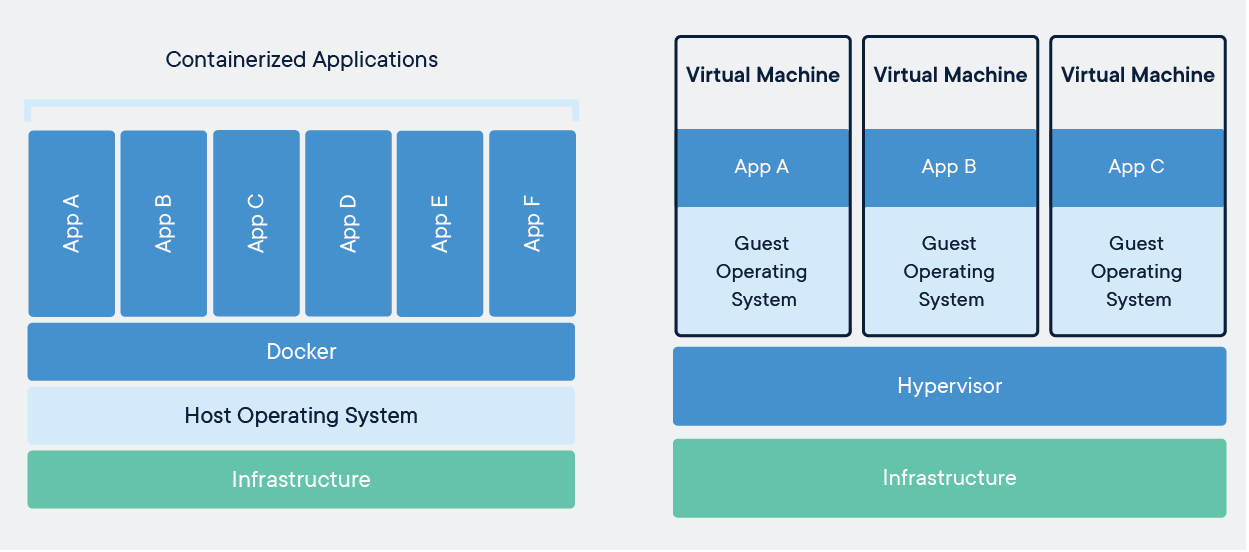
\includegraphics[scale = 0.25]{imgs/container-VM.png}
    \caption{Container and Virtual Machine}
    \label{fig:container_img}
\end{figure}

The web service, the search service, and the online shopping service are designed as simple static website services. Each service contains two network functions: a reverse proxy server and a static HTML web server. The reverse proxy increased the security by keeping the actual address of the backend server remains unknown to users. In this setup, the reverse proxy server just listens to the request from clients and forward it further to the server address. The web servers contain static HTML files which are different among the services. For example, the search service server contains a static HTML Google web page, the shopping service server contains a static HTML Amazon website, and the web service server contains a static HTML Wikipedia website. We can have several servers in the same node by assign each server to each different port as we can see in \ref{fig:metro_network_deployment}. In this case, we only deployed the proxy server in node 4 but noted that the proxy server also can be deployed at node 3 and node 2. All of these servers are built based on Nginx images in DockerHub.  

\begin{figure}[]
    \centering
    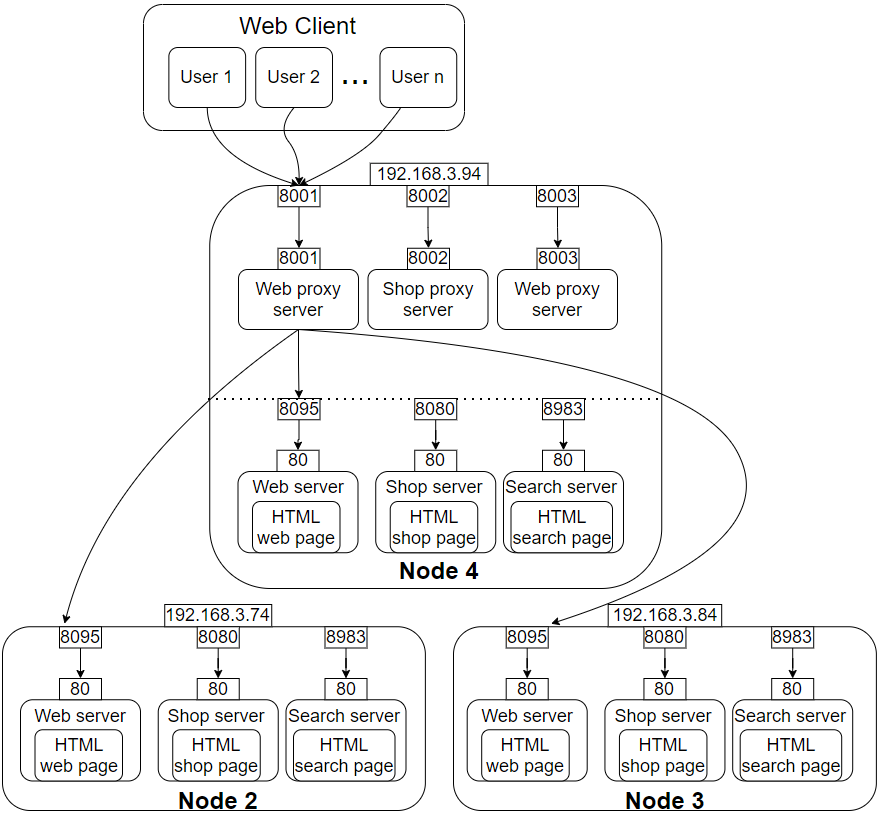
\includegraphics[scale = 0.36]{imgs/metro_network_deployment.png}
    \caption{Services and client deployment in MEC network}
    \label{fig:metro_network_deployment}
\end{figure}

\subsection{User generator}

Because the access network is not available in the lab, simulated traffic is generated from nodes to the metro network as client containers. To the most knowledge of the author, most of the user behavior can be assumed daily periodic based on research papers \cite{Kooti2016, Ullah2012, Taghavi2012, Yu2006}. Based on the patterns in these researches, a software program python-based has been constructed to simulate the user. To simulate multiple concurrent users at the same time we used multi-threading in python. Each thread represents a user. By changing the number of threads in the program, we can change the number of user requests to services. Because the service servers contain static HTML files, the amount of traffic will be proportional to the number of user requests. Therefore, the pattern of traffic captured over time in the research papers can be translated to the pattern of user number over time. 

\begin{figure}[]
    \centering
    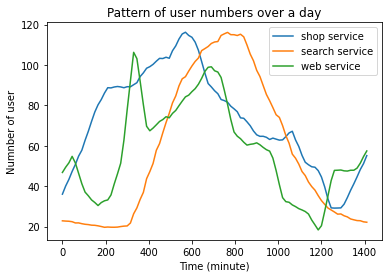
\includegraphics[scale = 0.55]{imgs/user_pattern_a_day.png}
    \caption{Number of user over a day according to traffic pattern in research papers}
    \label{fig:user_pattern}
\end{figure}

The client container takes two main parameters as input: the number of users and the service port number. By updating the number of users over time according to the traces from research papers, we can simulate the overall aggregated traffic. By adjusting the service port number, we can choose which service the client container subscribes to. User requests can come from any node and they can request any service in the network. Therefore, there can be multiple client containers in any node. Each client container can subscribe to any network service. For example, in the Figure \ref{fig:metro_network_deployment}, we consider a client container for web service. This client container contains $n$ threads, each thread represented a user. This number of threads can be updated as a global environment in the client container. Each thread requests the web service with the fixed request rate of 2 requests/sec via requests package in python library.

% section User traffic generation (end)


\section{Reinforcement learning agent design}
\label{sec:RL_Agent}
% section Reinforcement learning agent design (begin)
Briefly speaking, reinforcement learning deals with learning via interaction and feedback, or in other words learning to solve a task by trial and error. As we can see from Figure \ref{fig:RL_overview}, the agent is the learner and the decision-maker from the environment, where the agent learns and decides what actions to perform. An action belongs to a set of actions that the agent can perform and the state is the state of the agent in the environment. For each action selected by the agent, the environment provides a reward which usually is a scalar value. By observing and receiving reward from environment, the agent learn how to react to solve the problem in environment. 

\begin{figure}[]
    \centering
        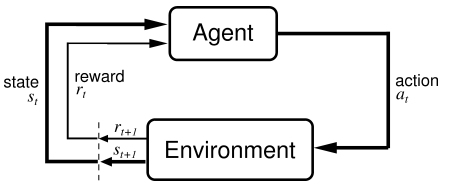
\includegraphics[scale = 0.6]{imgs/DRL.png}
        \caption{Agent-environment interaction}
        \label{fig:RL_overview}
    \end{figure}

In this section, the mathematical network model is presented in \ref{subsec:network_model}. To optimize the goal in the network model using the RL method, a Markov Decision Process (MDP) is proposed in \ref{subsec:POMDP}. Finally, an RL agent to solve the MDP is designed in section \ref{subsec:RL_design}.

\subsection{Network modelling}
\label{subsec:network_model}
The metro network is model as a graph $G = <N, L> $ with $N$ is the number of nodes and $L$ is the link between them. Each node $n \in N$ is modeled with its own amount of computing resource capacity $n_{cap}$ and each link $L$ is model with its own link delay depends on the length of the link $L_{delay}$. Each service $s \in S$ is model as a service chain function (SFC) which is combined from several virtual network functions (VNF) $vnf \in VNF$. For example, web service can be model as a service chain with proxy server and web server combine: $s_{search} = <vnf_{proxy server}, vnf_{server}>$. Moreover, service $s$ has its own service priority in the network. Each VNF has its own processing time for requests from clients. To model the clients for different services, the traces in \ref{sec:User traffic generation} are used. The traffic flow from client $f$ is modelled by client request rate $f_{rate}$ and which service it is requested $f_s$. The metric data are captured after every $\Delta$ time. The metrics that we captured are the statistic of latency, the number of dropped requests and successful requests of each SFC over the whole period, and the run time of the program. 

For traffic routing and VNF placement, the request routing table is introduced. The idea is the same with the scheduling table in \cite{9269087}. Each node in the MEC network has a traffic routing table we can see in Table \ref{tbl:traffic_routing}. Let us say the network has 3 nodes: node 2, node 3, and node 4. In node 2, we have incoming traffics from clients to several services such as search service and web service. According to Table \ref{tbl:traffic_routing}, when a search request coming to node 2 from the client and demand to be processed with $vnf_{proxy server}$, 50\% chance it will be processed at the proxy server of node 2 and 50\% chance it will be routed to node 3 processed at the proxy server of node 3. By doing this, it also does the provisioning where should the VNF be. For example, according to Table \ref{tbl:traffic_routing}, the web proxy server is only placed at node 2 in the entire network. To present the table in mathematical way, let us denote decision variable $x(n,s,vnf,n) | n \in N, s \in S, vnf \in VNF$. This variable decided how likely where a traffic flow should be served for each node, each service, and each VNF in that service. There are 2 constraints to this variable. To avoid fragmentation, it should have a minimum value $x_{min}$. The total percentage for a VNF should be 1.

\begin{table}[]
    \label{tbl:traffic_routing}
    \caption{Request routing table in node 2}
    \centering
    \begin{tabular}{|l|l|l|l|l|}
    \hline
    Service & VNF                 & Node 2 & Node 3 & Node 4 \\ \hline
    Search  & Search proxy server & 0.5    & 0.5    & 0      \\ \hline
            & Search server       & 0.33   & 0.33   & 0.33   \\ \hline
    Web     & Web proxy server    & 1      & 0      & 0      \\ \hline
            & Web server          & 0.5    & 0.5    & 0      \\ \hline
    ...     &                     &        &        &        \\ \hline
    \end{tabular}
\end{table}

We assume that the network function does not occupy any fixed computing resources. Therefore, the computing resource usage at each node $n_{used} \in [0, n_{cap}] | n \in N$ depends on the traffic load coming to the node and asked to be processed. In details, it depends on the request routing table (or $x(n,s,vnf,n)$) and user request data rate $f_{rate}$. A client flow is dropped if there is not enough capacity in the node.

The objective is to increase the quality of service for users, which is to satisfy the low latency and maximize the successful request rate. The latency is already be solved by edge computing. By correct rearrangement of the traffic routing table, we can maximize the successful request rate from users. To formulate the objective, we have the following equation: 

\begin{equation}
    \label{eqn:reward}
    % R = \frac{\sum succ_{sfc} priority_{sfc}}{2}
    O = \frac{\sum succ_{sfc} \times priority_{sfc} - \sum drop_{sfc} \times priority_{sfc}}{\sum succ_{sfc} \times priority_{sfc} + \sum drop_{sfc} \times priority_{sfc}}
\end{equation}

The objective $O$ calculates the successful request rate of all services over the $\Delta$ time. The higher the priority of service, the more that service contributes to the total success rate. By maximizing this term, it encourages the network to serve more the service requests from users, especially the high priority one.

\subsection{Markov Decision Process}
\label{subsec:POMDP}
A Markov Decision Process (MDP) is a mathematical framework used for modeling decision-making problems. It contains:

\textit{Observation space}: $O = {f_{rate}(n,s) | n \in N, s \in S}, {n_{used} / n_{cap} | n \in N}$. It observes the traffic flow from client at each node for each service and the utilization percentage of each node during the last $\Delta$ time. 

\textit{Action space}: $A = x(n,s,vnf,n) | n \in N, s \in S, vnf \in VNF$. The action space described the request routing table as in \ref{tbl:traffic_routing}. For each node, we have a particular traffic routing table and the action is to update the table after every $\Delta$ time. As we can see, the action space is continuous. 

\textit{Reward}: $R = O_{\Delta}$. We use the objective function but we calculate it only based on the last $\Delta$ time.

\subsection{RL design}
\label{subsec:RL_design}

The main idea here is that the RL agent observes new observations from metrics collected for the last $\Delta$ interval of time. Based on the monitored information and also the reward from the last action, it decides how to route the requests from each node to another. The RL agent is trained offline. During this time, it interacts with the environment and learns to give the best action given the observation. After training, it will be able to schedule where the requests should be served, allocate the IT resources accordingly. Because the action space in our MDP is a continuous space, a deep deterministic policy gradient (DDPG) algorithm is chosen \cite{Lillicrap2016}. DDPG is the algorithm that learns a deterministic policy and a Q-function by using each to improve the other. 

Action-value function Q:
It is good to know the total expected reward if the agent starts at a specific state $s$, takes an action $a$ and then takes the action according to the same policy $\pi$ until finish the trajectory $\tau$. This is the concept of action-value function $Q(s,a)$:

\begin{equation}
    \label{eqn:action-value}
    Q(s,a) = E_{\tau ~ \pi} [R(\tau) | s_0 = s, a_0 = a]
\end{equation}

To calculate the optimum action-value function $Q^*(s, a)$ we need to find the optimum policy which maximizes the action value-function: 

\begin{equation}
    \label{eqn:optimum-action-value}
    Q^*(s,a) = \max_{\pi} E_{\tau ~ \pi} [R(\tau) | s_0 = s, a_0 = a]
\end{equation}

If we know the optimum action-value function $Q^*(s, a)$, then in any given state, we can find the optimum action by: 

\begin{equation}
    \label{eqn:optimum-action}
    a^*(s) = \arg\max_{a} Q^*(s,a)
\end{equation}

As we can see in eqn. \ref{eqn:optimum-action-value} and \ref{eqn:optimum-action}, the agent interleaves learn both how to maximize the Q-function and action policy. 

The most difficult here is that this is works perfectly with the discrete action space because calculating $a^*(s)$ from Eqn \ref{eqn:optimum-action} is very straightforward. We just check and calculate with each action $a$ and chose the one that maximizes the term $Q^*(s, a)$. However, in our problem, the action is continuous, which means if we calculate the maximum normally, it required huge computation resources as well as calculation time. This is unacceptable since the agent acting in the environment and needs to respond to the environment in a fast manner. 

To solve this problem, DDPG comes up with an idea of learning a policy $\mu(s)$ to optimize the action to satisfy the maximum of $Q^*(s, a)$. Therefore, in steads of calculating $\max_{a} Q(s,a)$, we can just approximate it with $Q(s, \mu(s))$. In DDPG, this gradient-based learning rule for policy $\mu(s)$ is presented as actor network and the $Q(s, a)$ is presented as critic network. Both of them are neural networks.

\begin{figure}[]
    \centering
    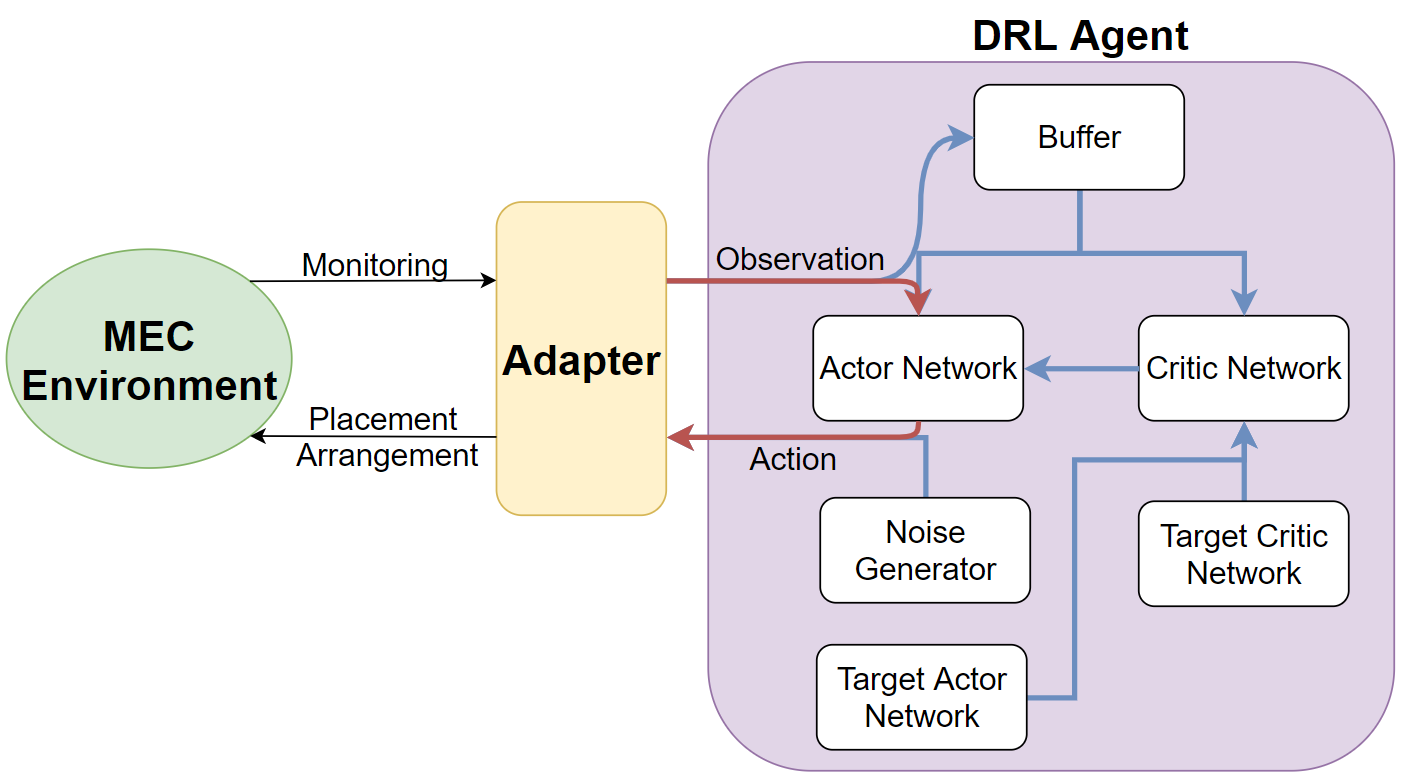
\includegraphics[scale = 0.23]{imgs/RL_design.png}
    \caption{The design of DDPG agent, the blue line represented the training process, the red line represented the testing process after training.}
    \label{fig:DDPG_design}
\end{figure}

\textit{Design}

The actor network $\mu(s)$ takes the observations as the input and gives the action at the output. In DDPG, the action is deterministic: $a = \mu(s)$. This means that with the same observation state, the output action is always the same. 

The critic network $Q(s,a)$ takes the observation and the action and gives out the Q-value as calculated in eqn. \ref{eqn:action-value}. The Q-value tells us how good the action is to maximize the long-term expected reward. The better the action, the higher the Q-value. The long-term reward is calculated as followed: $R(\tau) = \sum_{t=0}^{T} \gamma^t r_t$. Substitute this term into eqn. \ref{eqn:action-value}, we have the so-called Bellman equation for action-value function: 

\begin{equation}
    Q(s,a) = E_{s' ~ P} [r(s,a) + \gamma \times E_{\tau ~ \pi}[Q_{\pi}(s', a')]]
\end{equation}

and if the policy is optimum then we have: 

\begin{equation}
    \label{eqn:optimum_Bellman_Q_function}
    Q*(s,a) = E_{s' ~ P} [r(s,a) + \gamma \times max_{a'} [Q*(s', a')]]
\end{equation}

It said that the value of starting point is the reward from being there, plus the value of wherever the agent lands next.

\textit{Training}

To train the critic network and actor network, we use replay buffer $D$. It contains the experiences that the agent interacts with the environment. For each interaction, it stores a tuple which contains: observation, action, reward and next observation $(s,a,r,s') \in D$. These data then can be fed into the critic and the actor network for training. The size of the buffer is limited. Therefore, after it reaches its capacity it will discard the oldest values to store the new values. 

Let us say the set of parameters in actor network is $\theta$. We need to update these parameters to get the perfect set which should give us the best action given the observation. Training this actor network is very straight forward. Let say if we have already a well-trained critic network, we can just update the parameters to have the maximum Q-value at the critic network: 

\begin{equation}
    \theta = \max_\theta E_{s ~ D} [[Q^{\phi}(s, \mu(s))]]
\end{equation}

Let us denote the set of parameters in the critic network is $\phi$. We also would like to train this network by finding the best set of $\phi$ also. Let say we have an optimal actor network and it gives $\mu_\theta(s)$. We already know from the Bellman equation that the optimal Q-value is the reward plus the value comes from the optimal actor network in the next observation. Therefore, we will try to minimize the difference between the actual Q-value we have from the critic network (with the parameters $\phi$) and the optimal Q-value: 

\begin{equation}
    L(\phi, D) = E_{(s,a,r,s') \in D}  [(Q_\phi(s,a) - (r + \gamma Q_\phi(s',\mu_\theta(s'))))^2]  
\end{equation}

By doing this, we are trying to make the Q-function be more like its target. However, in this case, the set of parameters $\phi$ in both the actual Q-value and the target are the same. When we update the parameters, they move together which makes the loss minimization unstable and the training process is unlikely to converge. To solve this, DDPG and most other Q-learning methods come up with the idea of the target network. The target network will not share the same set of $\phi$ with the network but it will lag the first with some time delay. In DDPG, they use the soft copy to slowly update the parameters in the target network from the main network by some constant averaging: 

\begin{equation}
    \phi_{targ} = \rho \phi_{targ}  + (1- \rho) \phi
\end{equation}

The same idea applied to the critic network $\mu(s)$: 

\begin{equation}
    \theta_{targ} = \rho \theta_{targ}  + (1- \rho) \theta
\end{equation}

To summarize, to train the critic network, we need to use data from buffer $D$, with the Bellman equation \ref{eqn:optimum_Bellman_Q_function}, assume we have the optimal target actor network and we also have a target critic network, we update the parameter $\phi$ in the way to minimize the difference between main critic network and target critic network:

\begin{equation}
    L(\phi, D) = E_{(s,a,r,s') \in D}  [(Q_\phi(s,a) - (r + \gamma Q_{\phi_{targ}} (s',\mu_{\theta_{targ}}(s'))))^2]   
\end{equation}

The agent interleaves training the actor and critic network together. It updated the $\theta$ and $\rho$ together. When we update the actor network, we freeze the critic network and when we update the critic network, we freeze the target critic network and the target actor network. 

Because of deterministic policy, we need to come up with a way for exploration during training. In DDPG, we add noise in action. In the original paper of DDPG \cite{Lillicrap2016}, the noise generator is Ornstein–Uhlenbeck. However, according to recent papers, normal Gaussian white noise work perfectly fine and it is less complex than Ornstein–Uhlenbeck noise. 
% TODO: citation here! 

\textit{Testing}

After training, we remove the noise generator to have the best action for testing. New observations are passed directly to the actor network $\mu(s)$ to get the best action as we can see in the red line in \ref{fig:DDPG_design}.

% section Reinforcement learning agent design (end)

\section{Implementation}
\label{sec:Implementation}
% section Implementation (begin)
We design the setup to demonstrate how RL works in a real MEC network. But first, we need to design a complete MEC network environment for the RL agent to learn. We also need to design the adapter between the environment and the RL agent to do translating the action to the network and calculating reward, pre-process the monitoring data for the RL agent. At last, we will do the implementation of the RL agent.


\subsection{Metro edge computing network}

In this work, we assume there are optical links between the nodes and the bandwidth is unlimited in these links. In real life, we need to make sure there are links among these network nodes. However, in this work, the main target is to optimize the computing resources capacity in each node such as CPU. In future work, the RL agent can be expanded to optimize both computing resources in each node and bandwidth resources in each link. The bandwidth can be assigned according to the request routing table by using ONOS at each node.

To implement the idea of the request routing table, we use the Nginx server load balancers with weights that we called request routers. Based on the weights assigned to the request router, we can split the incoming requests accordingly. Therefore, when updating the request routing table in each node from the action of the RL agent, we update the weights in these request routers. The request router is also designed as a container and deployed in all nodes in the network. 

To monitor the drop requests and successful requests, round-trip time latency as well as node utilization, we used Prometheus. Prometheus will place the node exporter at each client container to scrape the metrics data and send them to the Prometheus server for storing and processing. This is where our adapter takes data and processes to give out the observations and reward to the RL agent. 

\begin{figure}[]
    \centering
    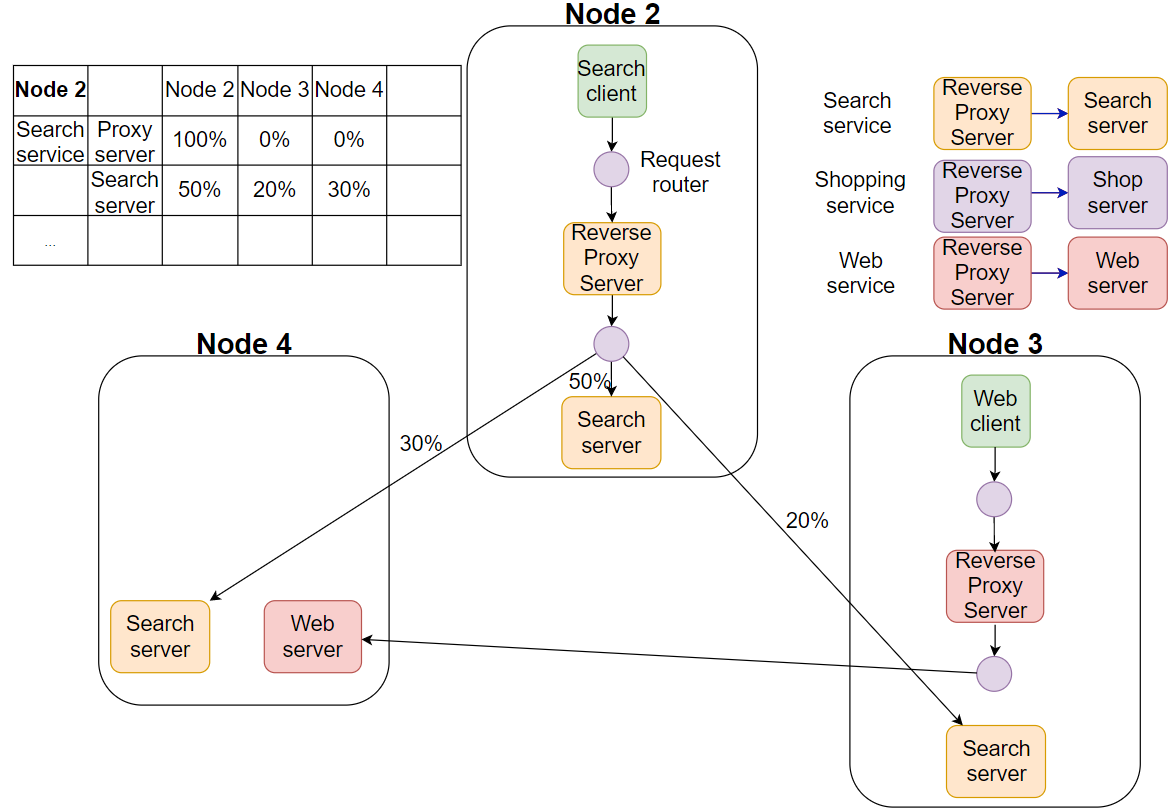
\includegraphics[scale = 0.28]{imgs/metro_network_env_client_services_router.png}
    \caption{The MEC network environment}
    \label{fig:metro_network_env_client_services_router}
\end{figure}

To demonstrate the capacity of the node, we set a limit request rate threshold zone. All servers in the same node use the same limit request zone. If the number of requests coming is higher than the threshold, it will be discarded. 

\subsection{Adapter}

To make the RL agent work in the MEC network, we need to design an adapter to translate action into a real setup as well as process the information from the MEC network into observation space and reward for RL to learn. As we can see in Figure \ref{fig:metro_network_adapter}, the Adapter captured the monitor data using the "Capture helper" class. This Capture Helper read data such as client request rate and server usage in Prometheus server, calculate the average them over $\Delta$ time, and translate them into observation space format for RL agent. On the other hand, it also passes the information about the dropped and successful request rate to the Reward calculator. After calculating the reward, together with the observation, the reward was also passed to the RL agent. The Capture Helper read the information from the Prometheus server continuously for an interval of $\Delta$ time. Then it sends the observation and reward after each interval time. 

When the Adapter received the action from the RL agent, we need to translate it into the request routing table. First of all, the action is pre-processed in the Action processor. There are two jobs here: to convert all action values which are lower than $x_{min}$ to 0 and to normalize the action according to each row in the request routing table to ensure the probability sum up to 1. After that, we update the weights in each request router at all nodes according to the action we got from the RL agent using docker. Moreover, we also need to update the user number in client containers according to the realistic trace. 

\begin{figure}[]
    \centering
    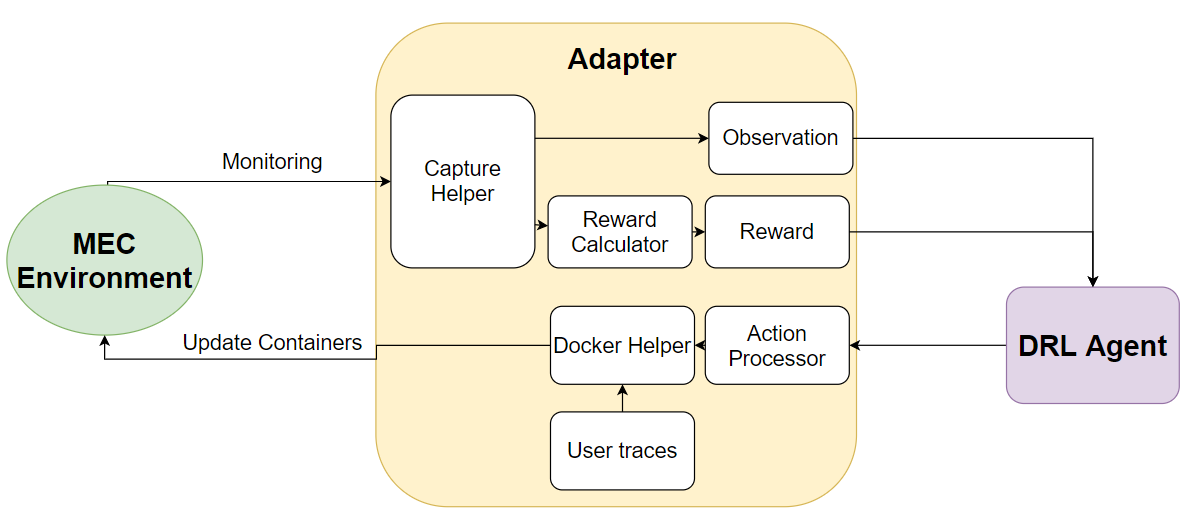
\includegraphics[scale = 0.28]{imgs/metro_network_adapter.png}
    \caption{The adapter design}
    \label{fig:metro_network_adapter}
\end{figure}

\subsection{RL Agent}
The Stable baselines 3 library with DDPG Agent for reinforcement learning framework is used to develop our DRL agent \cite{stable-baselines3}. In this design, we set the specify parameters: the actor network and critic network is designed with 1 hidden fully connected layer with 64 nodes, activation function for all node is ReLU function, discount factor for reward function is $\gamma = 0.99$, soft update for target network $\rho = 0.0001$ , learning rate $\alpha = 0.01$ , buffer size $D = 10000$ , noise variation for Gaussian white noise $\sigma = 0.2$, threshold $x_{min} = 0.1$ and learning start after 1 episode.

According to \cite{rlblogpost}, the reinforcement learning training outcome depends a lot on the random seed. Therefore, with different seeds in the beginning as initial, we can have very different results in reinforcement learning. We should run multiple times with different seeds to find the best solution with a particular seed. In this implementation, we run training in each case 10 times and chose the best for testing. 
% section Implementation (end)

\section{Evaluation}
\label{sec:Evaluation}
% section Evaluation (begin)
\subsection{Simulation}
In this work, we develop the network simulator from the simulator in \cite{9269087}. It can simulate the network nodes, links, service chain with network functions and user traffic flows as we discussed in \ref{sec:RL_Agent}. However, we need to modify it to fit our problem. First, we design the network graph topology based on our real setup in the lab. Second, we use the traces that we got from \ref{sec:User traffic generation} to simulate the user traffic pattern. Third, we designed multiple services feature in the simulator so it can deploy multiple services in the simulator's network. 

To implement the multiple-service feature, we need two data. We add up all user patterns for all services together to create a total arrival rate data-trace. Meanwhile, we create another data-trace that specifies how many percentages each service occupies at a specific time in the total arrival rate data-trace. After that, we put both traces as input to the network simulator. In the simulator, we designed a trace processor: for each incoming request from users, we based on the percentage data that we had to classify which service the request should subscribe to.

\subsection{Evaluation scenarios}
We evaluate the RL agent with simulation and our real MEC network. First, we evaluate the real MEC network topology with 3 nodes, each node with its computing capacity. We evaluate in 2 cases: the capacity is evenly distributed among 3 nodes and the capacity is unevenly distributed among 3 nodes. We also evaluate the case of multiple services (search, web, shopping) in our network with different priorities among them. Each client has its traffic pattern to its service. For simulation, we set the $\Delta = 100$ time steps and we set an episode that has 9600-time steps. For the MEC network, we set the $\Delta = 15$min and an episode is equal to a day with 96 $\Delta$ time intervals. The number and location of the client are fixed and do not change over time. Noted that the $\Delta$ is the time the DRL agent observes the environment before giving action. After that, we further investigate the scalability of the RL agent when we increase the number of nodes in a ring topology. We also further increase the number of clients in the metro network to evaluate the ability to handle multiple clients of the RL agent. 

\subsection{Experiment procedure}
In all scenarios, we always train in the simulation to get the well-trained model with different random seeds. Then we pick up the best model among them. After training, we save the model and test it (remove noise from action) in our MEC network to verify its ability in a real-life environment. This is way much faster than training in a real-life scenario. 

\subsection{Baseline algorithms}
For benchmark, we use simple baseline algorithms: load balancing and shortest path algorithm. These baseline algorithms are also used as benchmark algorithms in \cite{8485853} and \cite{9269087}. 

\textit{Load balancing:} Distribute the user requests to all node in the network which has capacity equally. This applies to all request routers in our network. This algorithm tries to balance the load among all nodes evenly to increase the throughput. 

\textit{Shortest path:} SP tries to minimize the number of network function instances in the network and latency. It places only 1 network function at a single node which closest to the traffic source. For example, it placed the first network function (reverse proxy server) at the node where the client requests come to the network and the next network function (server) at the closest node to it which has the capacity to deploy. It also favors the node which has a less number of network functions. 

\subsection{MEC network evaluation}
In the MEC network, we have a 3-node topology as we have seen in section \ref{sec:Implementation}. Firstly, we evaluate our model in two scenarios: distribute capacity equally and distribute capacity unequally. Secondly, we evaluate our model with multiple services with different priorities. In both cases, we extensively train the model in simulation before applying the model in the MEC network. 

\textit{Different capacity distribution}
In the capacity distribute equally scenario, we set the capacity in all nodes with the same capacity of 200 requests/sec. We investigate with multiple-service trace with one service. We deployed the client containers in two nodes in the network as we can see in Figure \ref{fig:balance_capacity_scenario}.

\begin{figure}[]
    \centering
    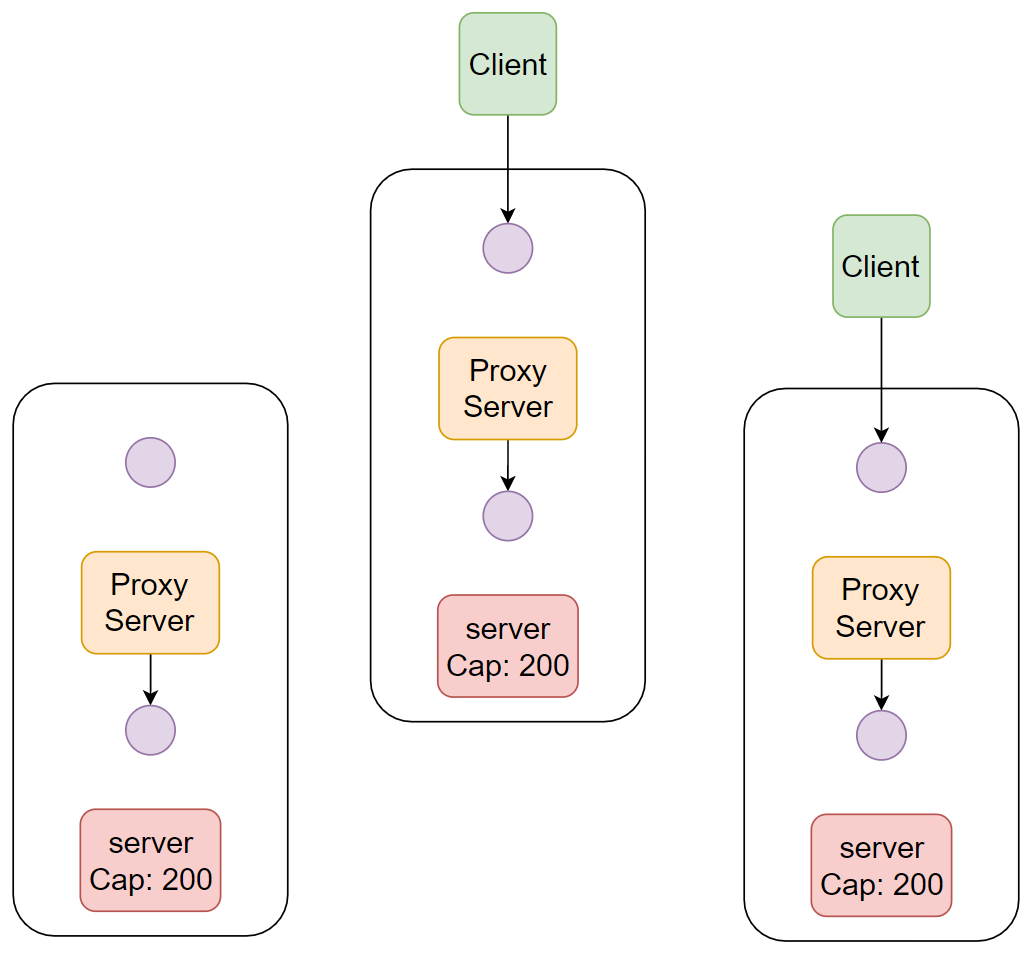
\includegraphics[scale = 0.5]{imgs/balance_capacity_scenario.png}
    \caption{The balance capacity scenario}
    \label{fig:balance_capacity_scenario}
\end{figure}

We peak at the solution of the RL agent at the time where the traffic is the highest in Figure \ref{fig:balance_capacity_RL_solution}. As we can see, it learns to put the traffic equally to all servers to fully utilize the resources in all nodes. This is a good sign that our RL agent learns and can work in the MEC network environment. 

\begin{figure}[]
    \centering
    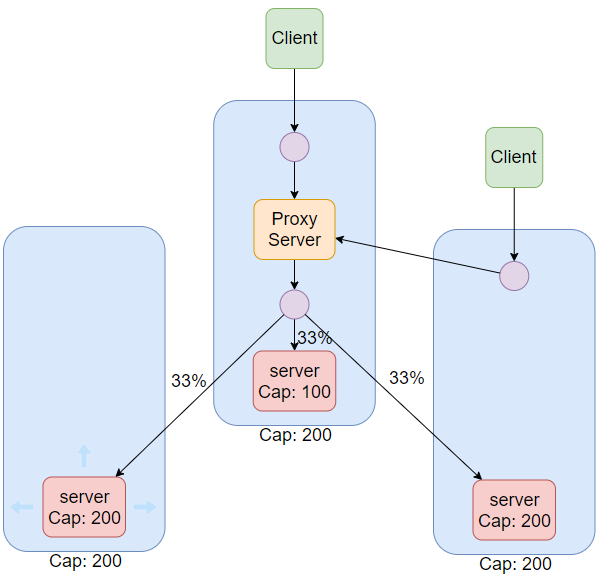
\includegraphics[scale = 0.5]{imgs/balance_capacity_RL_solution.png}
    \caption{The RL solution for balance capacity scenario}
    \label{fig:balance_capacity_RL_solution}
\end{figure}

In Figure \ref{fig:balance_capacity_scenario_result}, we can see that within a 1-day test, our RL agent performs better than other benchmark algorithms. The shape of the drop request rate is quite similar to the trace pattern. It is understandable since the higher the request rate from the user, the faster the node capacity gets full and the higher the drop request rate.
%TODO: ans question: buffer in server? what is the rate of user? max 200 + 200 = 400 why total cap of 600 can not fullfill this? 
% Why the load balance is not as good as RL agent? 

\begin{figure}[]
    \centering
    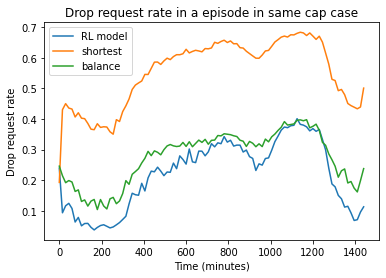
\includegraphics[scale = 0.5]{imgs/balance_capacity_scenario_result.png}
    \caption{The drop request rate in a day tested in real MEC network environment with balance capacity scenario}
    \label{fig:balance_capacity_scenario_result}
\end{figure}

In the capacity distribution unequally scenario, we decrease the capacity in node 3 with only 100 requests per second as we can see in Figure \ref{fig:unbalance_capacity_RL_solution}. We also look at the solution of our model when the traffic rate is the highest. It showed that the RL agent distributed the traffic accordingly to the node capacities ratio.

\begin{figure}[]
    \centering
    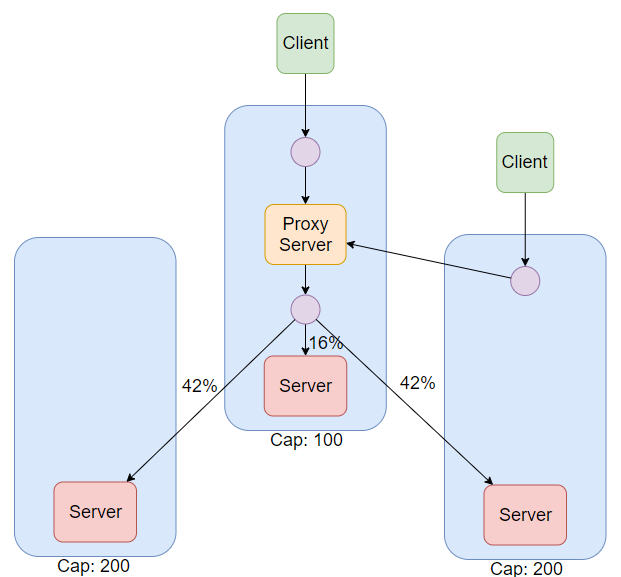
\includegraphics[scale = 0.5]{imgs/unbalance_capacity_RL_solution.png}
    \caption{The RL solution for unbalance capacity scenario}
    \label{fig:unbalance_capacity_RL_solution}
\end{figure}

As we can see in figure \ref{fig:unbalance_capacity_results}, it also proves that our RL model outperforms other baseline algorithms. Because the capacity distribution is unevenly among the nodes, the load balance algorithm is not as good as the one in \ref{fig:balance_capacity_scenario_result}. The result in both cases proves that our RL model can adapt to different types of capacity distribution scenarios.

We also notice that the average drop request rate (in our RL algorithm) increases when we reduce the total capacities in the network from $21.9\%$ in the balance case to $24.7\%$ in the unbalanced case. This happened because we reduce the capacity in the node. Therefore, requests get discarded.

\begin{figure}[]
    \centering
    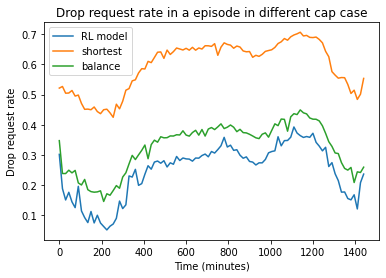
\includegraphics[scale = 0.5]{imgs/unbalance_capacity_results.png}
    \caption{The drop request rate in a day tested in real MEC network environment with unbalance capacity scenario}
    \label{fig:unbalance_capacity_results}
\end{figure}

\textit{Multiple services with priority}
In this experiment, we used multiple services in our training then applied them in the MEC network. We use the scenario of unbalanced capacity distribution. As we can see in Figure \ref{fig:multiple_service_scenario}, the clients which request three services (search service, web service, and shop service) are deployed in node 3 and node 2. The priority we set for search service, web service, and shop service are 7, 2, and 1, respectively. 

\begin{figure}[]
    \centering
    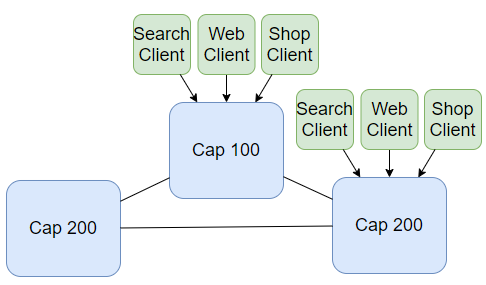
\includegraphics[scale = 0.5]{imgs/multiple_service_scenario.png}
    \caption{The multiple service scenario}
    \label{fig:multiple_service_scenario}
\end{figure}

As we can see in Figure \ref{fig:multiple_service_drop_request_rate_result}, it showed the drop request rate for different services in our MEC network. It showed that the RL agent learns how to prioritize the higher priority service. In this case, even though the overall drop request rate of our RL model is not as good as the load balance algorithm, the highest priority service (search service) does perform significantly better with the lowest drop rate request. Noted that the other services suffer higher dropped rate. In the case of shop service, it even performed worse than the load balance algorithm. To sum up, the RL agent learns to prioritize to serve the important service. 

\begin{figure}[]
    \centering
    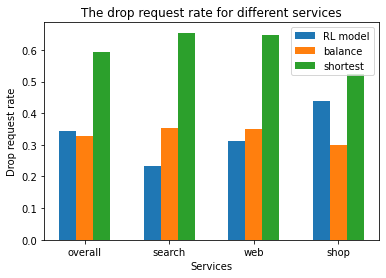
\includegraphics[scale = 0.5]{imgs/multiple_service_drop_request_rate_result.png}
    \caption{The drop request rate in multiple services case}
    \label{fig:multiple_service_drop_request_rate_result}
\end{figure}

\subsection{Scalability evaluation}
To test the scalability of the RL agent, we increase the network size in our simulation and test if our RL agent can provide a good solution in such a case. We also evaluate the case when the number of clients increases in the network given that the network also increases capacity to provide for those clients.

\textit{Increase network size}
We increase the network size from 3 nodes to 6, 8, 12, and 16 nodes. When we scaling, each node in the network has a random capacity but the total capacity of all nodes is the same. The client number is keeping the same in all cases. As we can see in Figure \ref{fig:drop_request_rate_diff_topology}, the RL model still outperforms other baseline algorithms, the drop rate increases when we increase the ring size. This is understandable since the more node, the more action space the RL model has. Therefore it will take more time for the RL agent to learn to find the best result. It might get stuck to the local minima point and take more training time to explore a better solution. As we can see in Figure \ref{fig:reward_different_topology}, the more complex topology takes more time and receive less reward in training to converge than the simple one. This explained why the complex ring size got a higher dropped request rate. We also noted that the running time for the RL agent increases as the network ring size increases as we can see in Figure \ref{fig:runtime_topology}. This is because when we increase the network size, the increase action space, we increase the parameters in actor neural network and critic neural network in RL model. Therefore, it takes a longer time to make a decision. But still, the decision is in a fast manner (milliseconds) compare to the monitoring interval $\Delta$ = 15 minutes.

\begin{figure}[]
    \centering
    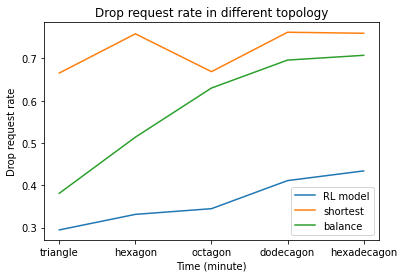
\includegraphics[scale = 0.5]{imgs/drop_request_rate_diff_topology.png}
    \caption{The drop request rate when increase the network size}
    \label{fig:drop_request_rate_diff_topology}
\end{figure}

\begin{figure}[]
    \centering
    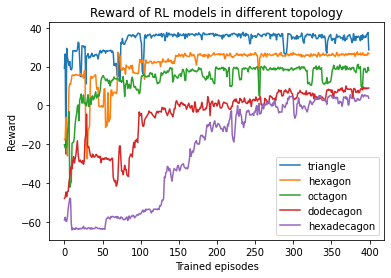
\includegraphics[scale = 0.5]{imgs/reward_different_topology.png}
    \caption{The RL reward convergence during training for different network size}
    \label{fig:reward_different_topology}
\end{figure}

\begin{figure}[]
    \centering
    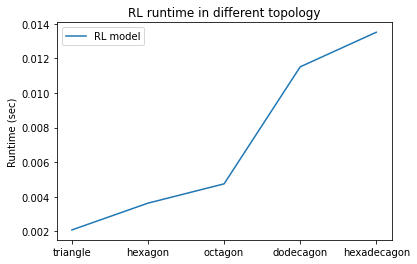
\includegraphics[scale = 0.5]{imgs/runtime_topology.png}
    \caption{The run time of RL model in different network size}
    \label{fig:runtime_topology}
\end{figure}

\textit{Increase clients}
In the last case, we would like to investigate the case when the number of aggregated traffic in the network increases from 2 to 8 in the 8-node network. The client placement in the network is random. The total capacity in the network increase as the number of client increase to make sure we have enough capacity for such clients. The capacity distribution in the metro network is random. As we can see in Figure \ref{fig:increase_ingress_clients}, the most important thing is that the RL model is to be able to keep the drop request rate low despite the number and location of clients as long as we provide enough total capacity in the metro network. On the other hand, other algorithms depend on the location of clients and how the total capacity is distributed in the network.

\begin{figure}[]
    \centering
    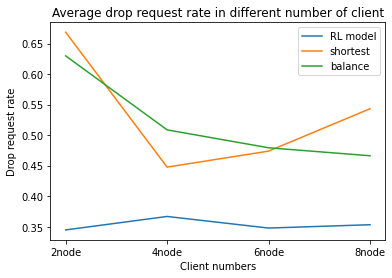
\includegraphics[scale = 0.5]{imgs/increase_ingress_clients.png}
    \caption{The drop request rate when increase number of clients}
    \label{fig:increase_ingress_clients}
\end{figure}

% section Evaluation (end)


\section{Conclusion}
\label{sec:Conclusion}
% section Conclusion (begin)
We have demonstrated that the reinforcement learning-based algorithm can be used to solve the resource utilization problem. It proves that with the good traffic arrangement solution from RL agent, the dropped request rate can be minimized. This achievement together with low latency from edge computing technologies can give a good quality of service to end-users in MEC network for services in 5G and beyonds.
% section Conclusion (end)

\bibliographystyle{IEEEtran}
\bibliography{ref/refs.bib}

\end{document}
